\setlength{\parskip}{\baselineskip}
\section[Theoretical Modeling]{Theoretical Modeling \& Robustness Analysis}

\begin{frame}
	\huge Theoretical Modeling \& Robustness Analysis
\end{frame}

\begin{frame}{PyTorch, C/C++, MATLAB}
	PyTorch $\rightarrow$ pure Python $\rightarrow$ C/C++ \& MATLAB
	\begin{itemize}
		\item Replicate PyTorch functionality
		\item Evaluation using PyTorch
		\item PyTorch pre-build \& pretrained AlexNet as a reference
		\item 2500 images of Kaggle cats \& dogs database
		\item Better understanding of underlining algorithms
		\item Explore Hardware implementation opportunities
		\item Quantization techniques $\rightarrow$ reduce memory footprint
		\item Algorithmic optimizations
		\item Minimize hardware resources and optimize performance using various tools
	\end{itemize}
\end{frame}

\begin{frame}{Algorithms}
	\begin{itemize}
		\item Convolution Layer
		\item Max-Pooling Layer
		\item Fully-Connected Layer
		\item ReLU
		\item SoftMax
	\end{itemize}
\end{frame}

\begin{frame}
	\center{\huge Memory Footprint}
	\begin{itemize}
		\item Classic hardware architectures $\rightarrow$ Compute bound
		\item ASICs \& FPGAs $\rightarrow$ Memory bound
		\item Highest benefit: Memory requirements fit into BRAM (order of MBs)
		\item Otherwise, external memory used $\rightarrow$ latency \& IO stalls
		\item Goal: Minimize memory footprint \& bandwidth
	\end{itemize}
\end{frame}

\begin{frame}{Memory Footprint: AlexNet Parameters (float32)}
	\begin{table}[H]
		\centering
		\begin{tabular}{llll}
			\toprule
			\textbf{Layer} & \textbf{\#Parameters}        & \textbf{Footprint} & \textbf{Memory (\%)} \\
			\midrule
			Conv1          & $64 * 3 * 11 * 11 = 23232$   & 92.92KB            & 0.04                 \\
			Conv2          & $192 * 64 * 5 * 5 = 307200$  & 1.22MB             & 0.5                  \\
			Conv3          & $384 * 192 * 3 * 3 = 663552$ & 2.65MB             & 1.09                 \\
			Conv4          & $256 * 384 * 3 * 3 = 884736$ & 3.53MB             & 1.45                 \\
			Conv5          & $256 * 256 * 3 * 3 = 589824$ & 2.35MB             & 0.97                 \\
			FC1            & $9216 * 4096 = 37748736$     & 150.99MB           & 61.79                \\
			FC2            & $4096 * 4096 = 16777216$     & 67.10MB            & 27.46                \\
			FC3            & $4096 * 1000 = 4096000$      & 16.38MB            & 6.70                 \\
			\midrule
			\textbf{Total} & 61090496                     & 244.36MB           & 100                  \\
			\bottomrule
		\end{tabular}
	\end{table}
\end{frame}

\begin{frame}{Memory Footprint: AlexNet Data Stages (float32)}
	\begin{table}[H]
		\small
		\centering
		\scalebox{0.9}{
			\begin{tabular}{llll}
				\toprule
				\textbf{Layer} & \textbf{\#Data}          & \textbf{Footprint} & \textbf{Memory (\%)} \\
				\midrule
				Image          & $3 * 224 * 224 = 150528$ & 150.52KB           & 6.07                 \\
				Conv1          & $64 * 55 * 55 = 193600$  & 774.40KB           & 31.22                \\
				MaxPool1       & $64 * 27 * 27 = 46656$   & 186.62KB           & 7.52                 \\
				Conv2          & $192 * 27 * 27 = 139968$ & 559.87KB           & 22.57                \\
				MaxPool2       & $192 * 13 * 13 = 32448$  & 129.79KB           & 5.23                 \\
				Conv3          & $384 * 13 * 13 = 64896$  & 259.58KB           & 10.46                \\
				Conv4          & $256 * 13 * 13 = 43264$  & 173.05KB           & 6.98                 \\
				Conv5          & $256 * 13 * 13 = 43264$  & 173.05KB           & 6.98                 \\
				MaxPool3       & $9216$                   & 36.86KB            & 1.49                 \\
				FC1            & $4096$                   & 16.38KB            & 0.66                 \\
				FC2            & $4096$                   & 16.38KB            & 0.66                 \\
				FC3            & $1000$                   & 4KB                & 0.16                 \\
				\midrule
				\textbf{Total} & 682856                   & 2.48MB             & 100                  \\
				\bottomrule
			\end{tabular}
		}
	\end{table}
\end{frame}

\begin{frame}{Memory Footprint Reduction}
	\begin{itemize}
		\item Data type bit-width shortening (float64-float16)
		\item Simpler data types (fixed-point/integers)
		\item Binary
		\item Quantization
		\item Quantization aware training
		\item Compression
		\item K-Means clustering
		\item Second Level Codebook
	\end{itemize}
\end{frame}

\begin{frame}{Memory Footprint Reduction}
	\center{\huge Trading accuracy to performance.}
\end{frame}

\begin{frame}{Memory Footprint Reduction: Evaluation}
	\begin{itemize}
		\item Baseline: PyTorch pre-trained pre-build AlexNet model
		\item Inferencing 2500 pre-transformed Kaggle cats \& dogs images
		\item Top-1 error rate
		\item MATLAB implementation used
		\item PyTorch \& C/C++ do not support half-floating point
	\end{itemize}
\end{frame}

\begin{frame}{Memory Footprint Reduction: Floating Point}
	\centering
	\large{Convert 32-bit floats to their closest representation.}
	\begin{table}[H]
		\centering
		\begin{tabular}{p{2cm} p{2cm} p{3cm} p{3cm}}
			\toprule
			\textbf{Tool} & \textbf{Data type} & \textbf{Top-1 Error rate (\%)} & \textbf{Avg. inference time (sec)} \\
			\midrule
			PyTorch       & float64            & 0                              & 0.091                              \\
			PyTorch       & float32            & 0                              & 0.034                              \\
			MATLAB        & float64            & 0                              & 6.624                              \\
			MATLAB        & float32            & 0                              & 8.162                              \\
			MATLAB        & float16            & 0.36                           & 147.480                            \\
			\bottomrule
		\end{tabular}
	\end{table}
\end{frame}

\begin{frame}{Memory Footprint Reduction: Fixed Point Parameters}
	\begin{itemize}
		\item Convert 32-bit float number sets to fixed-point
		\item Select best radix-point position to most accurately represent the number set
		\item Use same scale factor on whole set
		\item Every layer has its own scale factor
	\end{itemize}
	\center{$Position = argmin_{i=0}^{W}[\frac{\sum_{j=1}^{size(S)} |S_j - FixPtConvert(S_j, W, i)| }{size(S)}]$}
\end{frame}

\begin{frame}{Memory Footprint Reduction: Fixed Point Parameters}
	\begin{table}[H]
		\centering
		\begin{tabular}{p{2cm} p{2cm} p{3cm} p{3cm}}
			\toprule
			\textbf{Tool} & \textbf{Data type} & \textbf{Top-1 Error rate (\%)} & \textbf{Avg. inference time (sec)} \\
			\midrule
			MATLAB        & fixed64            & 0                              & 7.318                              \\
			MATLAB        & fixed32            & 0                              & 7.692                              \\
			MATLAB        & fixed16            & 22                             & 6.650                              \\
			MATLAB        & fixed14            & 28.44                          & 6.813                              \\
			MATLAB        & fixed12            & 36.24                          & 6.797                              \\
			MATLAB        & fixed10            & 77.07                          & 6.929                              \\
			MATLAB        & fixed8             & 100                            & 6.312                              \\
			\bottomrule
		\end{tabular}
	\end{table}
\end{frame}

\begin{frame}{Memory Footprint Reduction: Fixed Point Parameters}
	\begin{minipage}{0.6\textwidth}
		\centering
		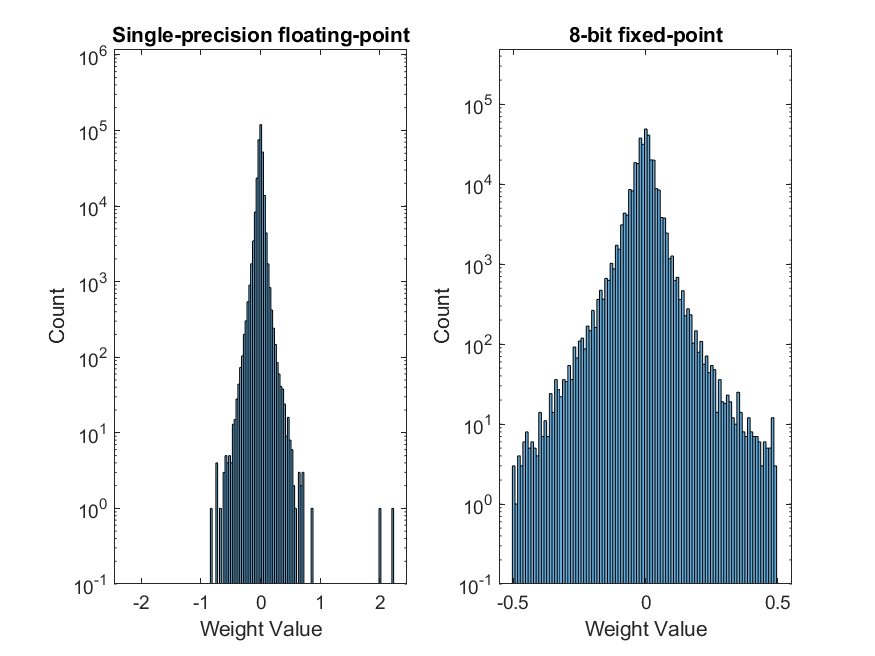
\includegraphics[width=0.95\textwidth]{../Images/Weights-distributions/original-vs-fixed8/weight-distribution-conv2.png}\\
	\end{minipage}%
	\begin{minipage}{0.4\textwidth}
		\large Histogram limits significantly altered\\
	\end{minipage}
\end{frame}

\begin{frame}{Memory Footprint Reduction: Fixed Point Parameters}
	\begin{minipage}{0.6\textwidth}
		\centering
		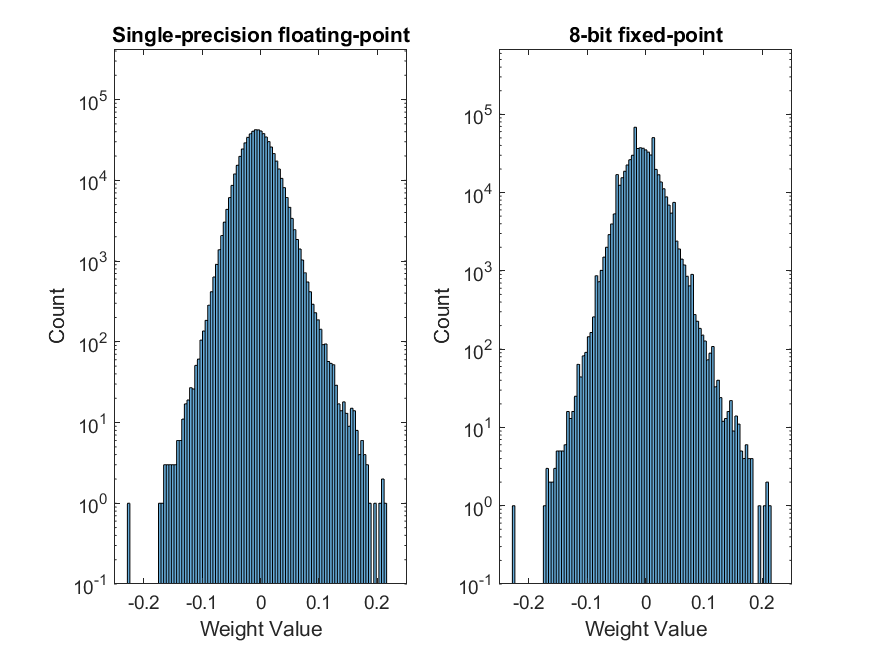
\includegraphics[width=0.95\textwidth]{../Images/Weights-distributions/original-vs-fixed8/weight-distribution-conv5.png}\\
	\end{minipage}%
	\begin{minipage}{0.4\textwidth}
		\large Significant spiking\\
	\end{minipage}
\end{frame}

\begin{frame}{Memory Footprint Reduction: Fixed Point Parameters}
	\begin{minipage}{0.6\textwidth}
		\centering
		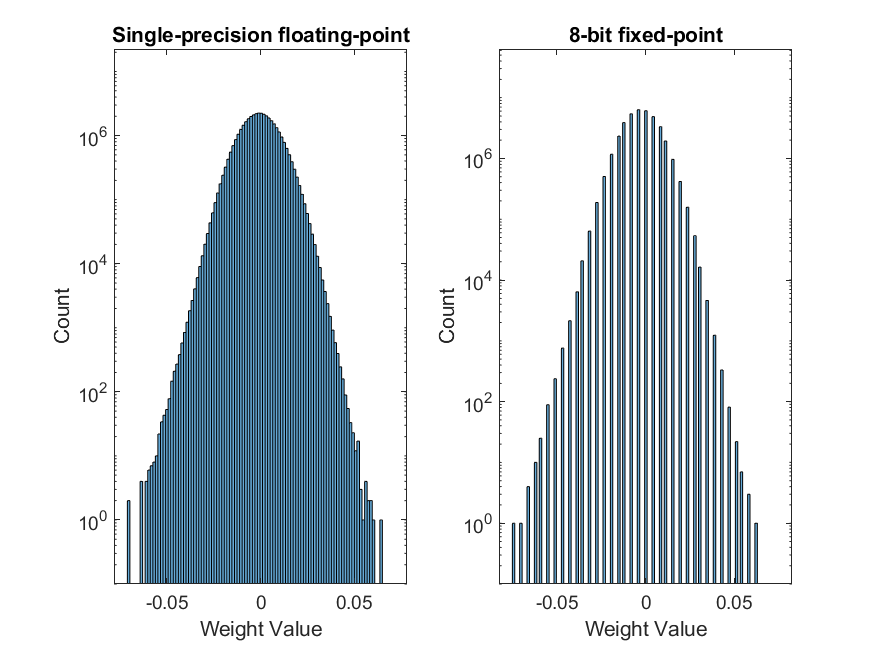
\includegraphics[width=0.95\textwidth]{../Images/Weights-distributions/original-vs-fixed8/weight-distribution-FC1.png}\\
	\end{minipage}%
	\begin{minipage}{0.4\textwidth}
		\large Severe subsampling\\
	\end{minipage}
\end{frame}

\begin{frame}{Memory Footprint Reduction: Fixed Point Parameters}
	\large{Use Mean Square Error (MSE)}\\
	$Position = argmin_{i=0}^{32}[\frac{\sum_{j=1}^{size(S)} |S_j - FixPtConvert(S_j, W, i)|^2 }{size(S)}]$

	\large{Use Mean Quarted Error (MQE)}\\
	$Position = argmin_{i=0}^{32}[\frac{\sum_{j=1}^{size(S)} |S_j - FixPtConvert(S_j, W, i)|^4 }{size(S)}]$
\end{frame}

\begin{frame}{Memory Footprint Reduction: Fixed Point MQE}
	\begin{table}[H]
		\centering
		\begin{tabular}{lll}
			\toprule
			\textbf{Tool} & \textbf{Data type} & \textbf{Top-1 Error rate (\%)} \\
			\midrule
			MATLAB        & fixed64            & 0                              \\
			MATLAB        & fixed32            & 0                              \\
			MATLAB        & fixed16            & 4.42                           \\
			MATLAB        & fixed14            & 17.59                          \\
			MATLAB        & fixed12            & 48.11                          \\
			MATLAB        & fixed10            & 86.91                          \\
			MATLAB        & fixed8             & 99.3                           \\
			\bottomrule
		\end{tabular}
	\end{table}
\end{frame}

\begin{frame}{Memory Footprint Reduction: Fixed Point Parameters}
	\begin{minipage}{0.6\textwidth}
		\centering
		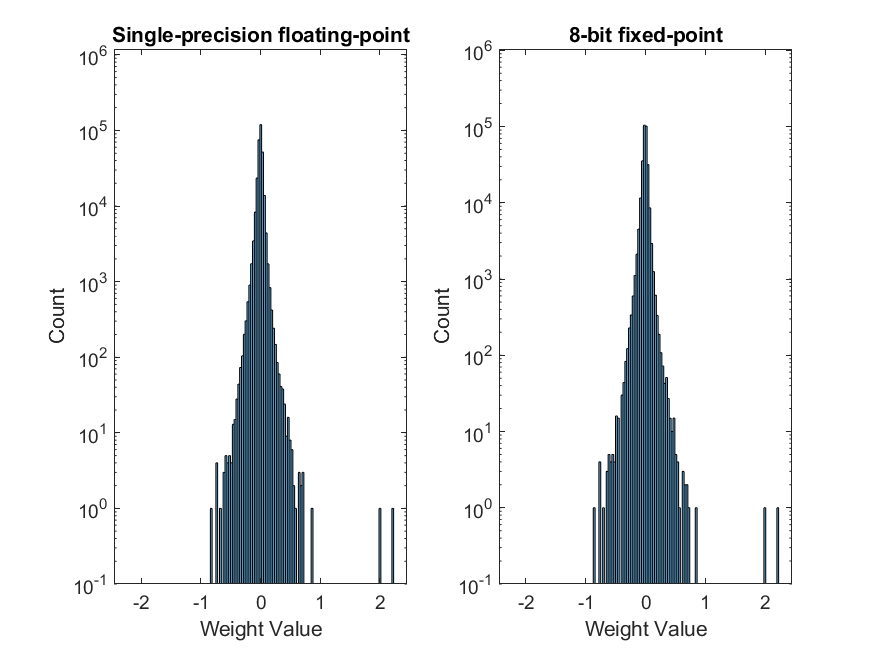
\includegraphics[width=0.95\textwidth]{../Images/Weights-distributions/original-vs-fixed8/weight-distribution-conv2-MQE.png}\\
	\end{minipage}%
	\begin{minipage}{0.4\textwidth}
		\large Histogram limits identical\\
	\end{minipage}
\end{frame}

\begin{frame}{Memory Footprint Reduction: Fixed Point Parameters}
	\begin{minipage}{0.6\textwidth}
		\centering
		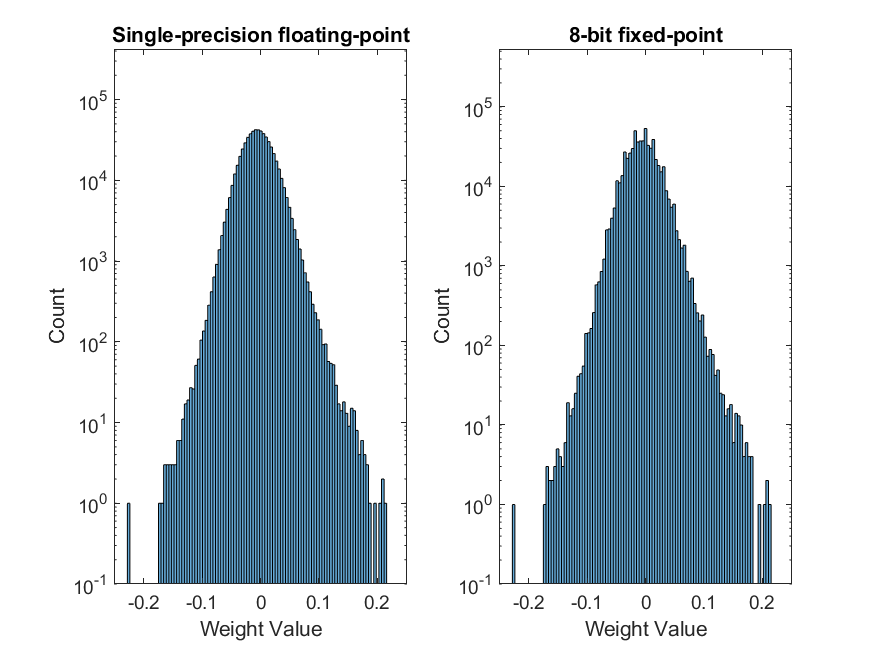
\includegraphics[width=0.95\textwidth]{../Images/Weights-distributions/original-vs-fixed8/weight-distribution-conv5-MQE.png}\\
	\end{minipage}%
	\begin{minipage}{0.4\textwidth}
		\large Slight spiking\\
	\end{minipage}
\end{frame}

\begin{frame}{Memory Footprint Reduction: Fixed Point Parameters}
	\begin{minipage}{0.6\textwidth}
		\centering
		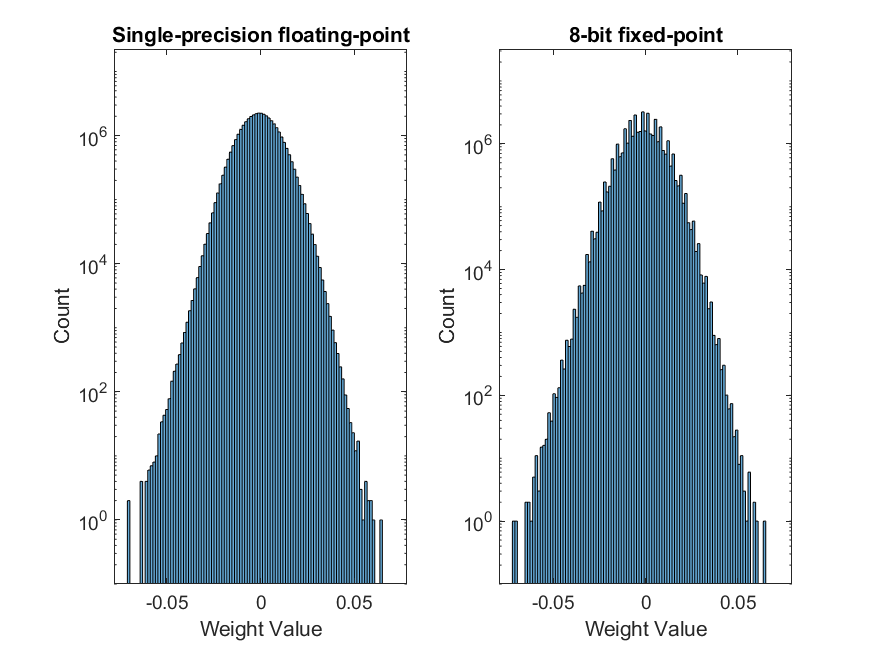
\includegraphics[width=0.95\textwidth]{../Images/Weights-distributions/original-vs-fixed8/weight-distribution-FC1-MQE.png}\\
	\end{minipage}%
	\begin{minipage}{0.4\textwidth}
		\large No subsampling, but spiking\\
	\end{minipage}
\end{frame}

\begin{frame}{Memory Footprint Reduction: All data types tested}
	\begin{minipage}{0.6\textwidth}
		\centering
		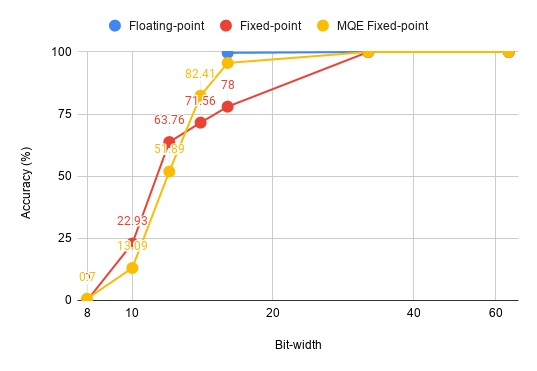
\includegraphics[width=0.9\textwidth]{../Images/Weights-distributions/data-types-accuracy-chart.png}\\
	\end{minipage}%
	\begin{minipage}{0.4\textwidth}
		\begin{itemize}
			\item Accuracy degradation is expected
			\item Model dependent
			\item Training dependent
		\end{itemize}
	\end{minipage}
\end{frame}

\begin{frame}{Memory Footprint Reduction: Fixed Point Activations}
	\begin{itemize}
		\item Floating-point arithmetic scales automatically
		\item Fixed-point activations may overflow
		\item Quantize every layer outputs
		\item Keep the upper N most significant bits to retain accuracy
		\item Finding on runtime the uppermost on is computationally intensive $\rightarrow$ any fixed-point benefits get obsolete
	\end{itemize}
\end{frame}

\begin{frame}{Memory Footprint Reduction: Fixed Point Activations}
	\centering
	\large{Calculate optimal activation scale factor per layer.}
	\newline
	\newline
	$Theoretical_{bitWidth} = input_{bitWidth} + weight_{bitWidth} + \lceil \log_2 \#Additions \rceil$
\end{frame}

\begin{frame}{Memory Footprint Reduction: Fixed Point Activations}
	\begin{minipage}{0.6\textwidth}
		\centering
		\begin{table}[H]
			\centering
			\begin{tabular}{lp{2cm}p{2cm}}
				\toprule
				\textbf{Layer} & \textbf{Theoretical bit-width} & \textbf{Practical bit-width} \\
				\midrule
				Input          & 8                              & 8                            \\
				Conv1          & 25                             & 17                           \\
				Conv2          & 27                             & 14                           \\
				Conv3          & 27                             & 15                           \\
				Conv4          & 28                             & 15                           \\
				Conv5          & 28                             & 17                           \\
				FC1            & 30                             & 17                           \\
				FC2            & 28                             & 17                           \\
				FC3            & 28                             & 17                           \\
				\bottomrule
			\end{tabular}
		\end{table}
	\end{minipage}%
	\begin{minipage}{0.4\textwidth}
		\begin{itemize}
			\item Theoretical worse case scenario significantly differs from practical
			\item Inference 2000 images, find maximum absolute valued activation per layer
			\item Maximum theoretical bit-width is 30-bits $\rightarrow$ all activations fit in 32-bit integers before quantization
		\end{itemize}
	\end{minipage}
\end{frame}

\begin{frame}{Memory Footprint Reduction: Fixed Point Activations}
	\begin{minipage}{0.6\textwidth}
		\centering
		\begin{table}
			\centering
			\begin{tabular}{llll}
				\toprule
				\textbf{Layer} & \textbf{Weights} & \textbf{Bias} & \textbf{Output} \\
				\midrule
				Input          & -7               & -             & -               \\
				Conv1          & -7               & -5            & -2              \\
				Conv2          & -5               & -7            & 0               \\
				Conv3          & -7               & -7            & 3               \\
				Conv4          & -8               & -6            & 5               \\
				Conv5          & -9               & -5            & 10              \\
				FC1            & -10              & -10           & 15              \\
				FC2            & -10              & -9            & 19              \\
				FC3            & -9               & -9            & 23              \\
				\bottomrule
			\end{tabular}
		\end{table}
	\end{minipage}%
	\begin{minipage}{0.4\textwidth}
		\large{Optimal scale factor per layer.}
	\end{minipage}
\end{frame}

\begin{frame}
	\center{\large Weight Pruning}
	\begin{itemize}
		\item Biological brain phase from birth until mid-20s
		\item Network compression
		\item Weak weights get pruned $\rightarrow$ $w \epsilon [-f, f] = 0$, f: pruning factor
		\item Calculations can get skipped
		\item Higher memory \& power efficiency \& inference performance
		\item Accuracy-Performance tradeoff
		\item Weight pruning amount varies per network
		\item Global pruning factor: Not a good idea!
	\end{itemize}
\end{frame}

\begin{frame}{Weight Pruning}
	\begin{table}[H]
		\centering
		\begin{tabular}{llll llll}
			\toprule
			\textbf{Layer}         & \textbf{Test 1} & \textbf{Test 2} & \textbf{Test 3} & \textbf{Test 4} & \textbf{Test 5} & \textbf{Test 6} & \textbf{Test 7} \\
			\midrule
			Conv1 (\%)             & 7.15            & 13.66           & 91.3            & 91.3            & 0               & 0               & 0               \\
			Conv2 (\%)             & 13.82           & 26.9            & 95.83           & 95.83           & 0               & 0               & 0               \\
			Conv3 (\%)             & 13.54           & 26.63           & 98.62           & 98.62           & 0               & 0               & 0               \\
			Conv4 (\%)             & 15.32           & 29.99           & 93.14           & 93.14           & 0               & 0               & 0               \\
			Conv5 (\%)             & 15.55           & 30.53           & 94.02           & 94.02           & 0               & 0               & 0               \\
			FC1 (\%)               & 41.23           & 41.23           & 41.23           & 94.48           & 41.23           & 71.89           & 96.61           \\
			FC2 (\%)               & 36.69           & 36.69           & 36.69           & 90.61           & 36.69           & 62.52           & 90.61           \\
			FC3 (\%)               & 27.27           & 27.27           & 27.27           & 89.68           & 27.27           & 47.74           & 75.56           \\
			\midrule
			\textbf{Total (\%)}    & 37.97           & 38.54           & 41.22           & 93.11           & 37.38           & 64.79           & 89.65           \\
			\midrule
			\textbf{Accuracy (\%)} & 91.74           & 80.8            & 0               & 0               & 90.87           & 71.77           & 15.06           \\
			\bottomrule
		\end{tabular}
	\end{table}
\end{frame}

\begin{frame}{Weight Pruning}
	\begin{minipage}{0.6\textwidth}
		\centering
		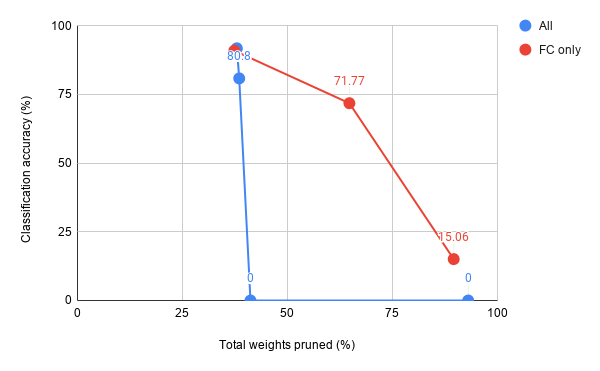
\includegraphics[width=\textwidth]{../Images/Weights-distributions/pruned/pruning-amount-vs-accuracy-chart.png}\\
	\end{minipage}%
	\begin{minipage}{0.4\textwidth}
		\begin{itemize}
			\item Less Pruning $\rightarrow$ Higher Accuracy
			\item Convolution layers more prone to error
			\item Pruning also denoises - Low valued weights act as noise
		\end{itemize}
	\end{minipage}
\end{frame}

\begin{frame}{Weight Pruning}
	\begin{minipage}{0.6\textwidth}
		\centering
		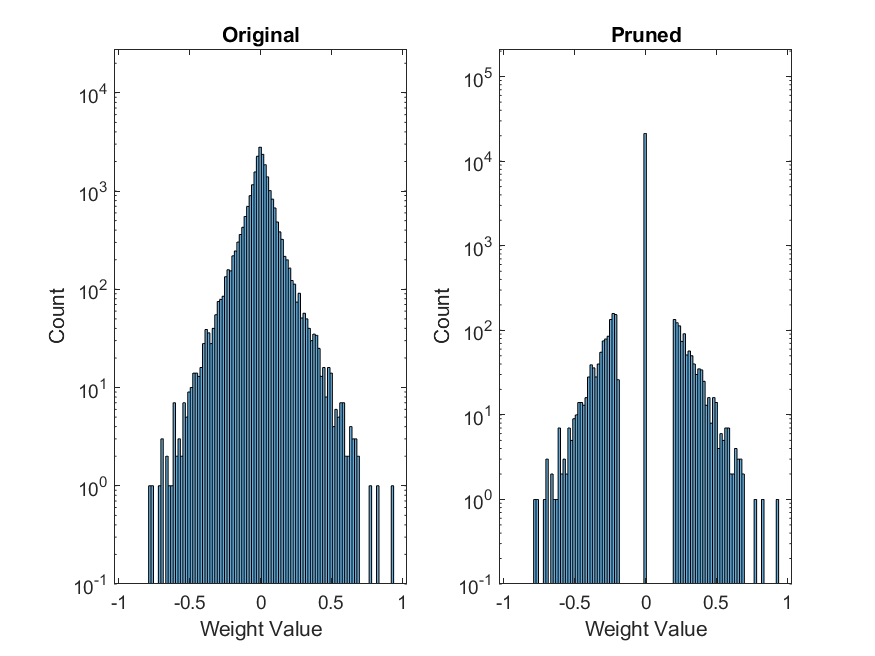
\includegraphics[width=\textwidth]{../Images/Weights-distributions/pruned/41.22/weight-distribution-conv1.png}\\
	\end{minipage}%
	\begin{minipage}{0.4\textwidth}
		\begin{itemize}
			\item Aggressive pruning
			\item High concentration of zeroes
			\item High compression factor
			\item Severe absence of near-to-zero valued weights
		\end{itemize}
	\end{minipage}
\end{frame}

\begin{frame}{Weight Pruning}
	\begin{minipage}{0.6\textwidth}
		\centering
		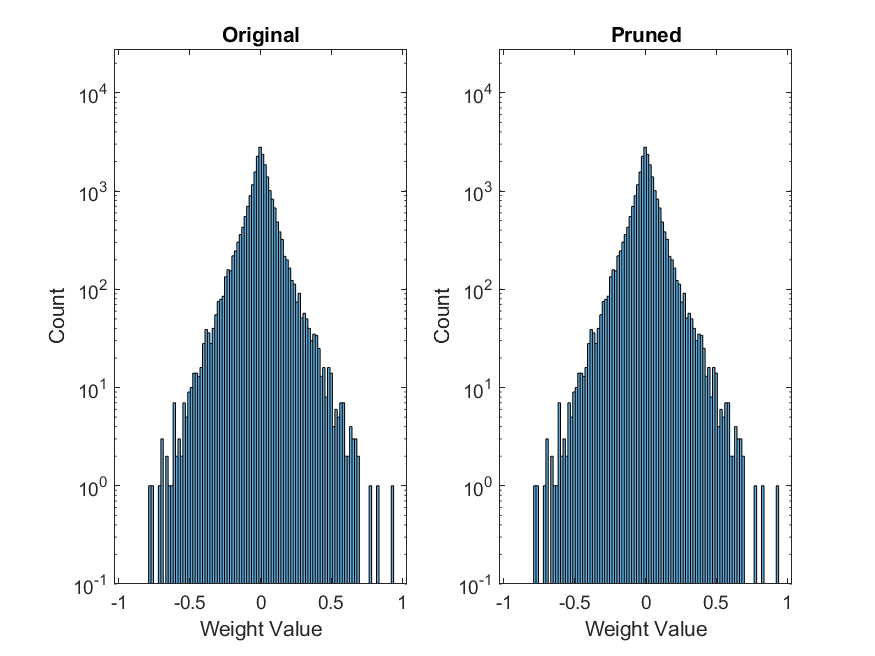
\includegraphics[width=\textwidth]{../Images/Weights-distributions/pruned/37.97/weight-distribution-conv1.png}\\
	\end{minipage}%
	\begin{minipage}{0.4\textwidth}
		\begin{itemize}
			\item Fine-tuned pruning
			\item Normal concentration of zeroes
			\item No discontinuation
		\end{itemize}
	\end{minipage}
\end{frame}
